\documentclass[11pt]{article}
\usepackage[margin=2.3cm]{geometry}
\usepackage{amsmath,amssymb}
\usepackage{booktabs,tabularx}
\usepackage{enumitem}
\usepackage[dvipsnames]{xcolor}
\usepackage{tikz}
\usetikzlibrary{arrows.meta,positioning}
\usepackage[colorlinks=true,linkcolor=MidnightBlue,urlcolor=MidnightBlue]{hyperref}
\setlist{itemsep=1pt,topsep=3pt}
\setlength{\parskip}{4pt}\setlength{\parindent}{0pt}

% evidence-status tags
\newcommand{\have}{\textsf{\small\textcolor{ForestGreen}{[have]}}}
\newcommand{\rerun}{\textsf{\small\textcolor{BurntOrange}{[re-run]}}}
\newcommand{\new}{\textsf{\small\textcolor{BrickRed}{[new]}}}
\newcommand{\thy}{\textsf{\small\textcolor{RoyalPurple}{[theory]}}}
\newcommand{\fig}[1]{\textbf{Fig.~#1}}
\newcommand{\tab}[1]{\textbf{Tab.~#1}}
\newcommand{\E}[1]{\textsf{\small E#1}}

\title{\textbf{Paper outline (JCP)}\\[4pt]
\large Continuous coordinate-network bases for Petrov--Galerkin reduced models:\\
deployment-time tunability and classical-quadrature hyper-reduction}
\author{Working outline, 2026-10-06 \quad---\quad planning document, no new results}
\date{}

\begin{document}
\maketitle

\noindent\fbox{\parbox{\dimexpr\linewidth-2\fboxsep-2\fboxrule}{\small
\textbf{How to read this.} Every item is tagged with its evidence status:
\have\ exists at full scale and can be reused once re-scored;
\rerun\ exists but must be redone under the new protocol (second-order references, sealed cohorts);
\new\ not yet run; \thy\ an analysis to write.
Experiment ids \E{0}--\E{9} refer to \S\ref{sec:exp}.
No numbers are given: all paper numbers will be generated from run JSONs.
Sources: \texttt{reports/2026-10-06-jcp-offmesh-paper-plan.md} and its appendices, the
discarded ICLR manuscript \texttt{paper\_latex/main.tex}, and Hari's off-mesh quadrature study.}}

\section*{One-sentence thesis}
A reduced trial basis that is a \emph{continuous, importance-ordered} function of position,
$u(x)=G(x)c$, gives two properties no mesh-bound basis has.
\textbf{(i)~Ordered:} a single trained model exposes an accuracy/cost dial at deployment, by choosing the bank width $R'$ and whether the nonlinear head is used.
\textbf{(ii)~Continuous:} the nonlinear term is an integral, so it can be hyper-reduced by \emph{classical} quadrature rather than by quadrature fitted to snapshots on the mesh. This removes per-mesh fitting and the mesh stencil's consistency error.

\begin{center}
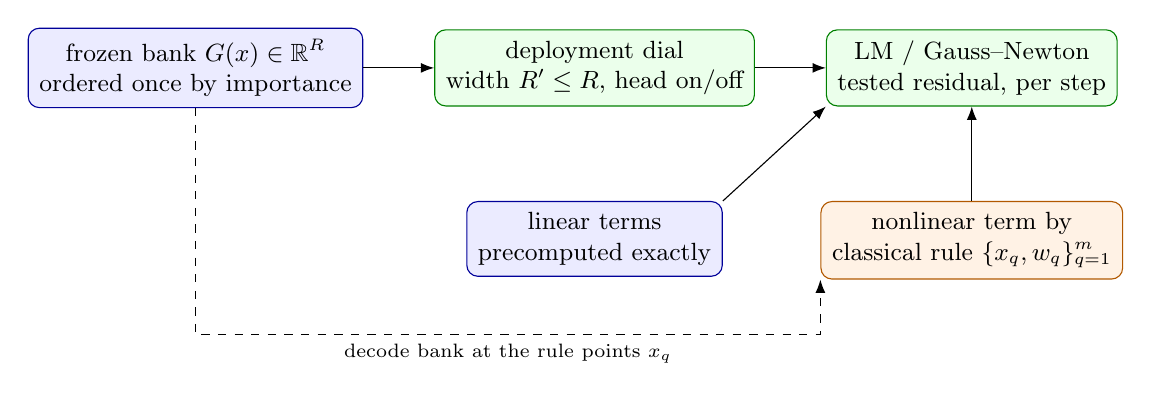
\begin{tikzpicture}[node distance=6mm and 9mm, every node/.style={font=\small,align=center},
 box/.style={draw,rounded corners,minimum height=9mm,inner sep=4pt},
 frozen/.style={box,fill=blue!8,draw=blue!60!black},
 solved/.style={box,fill=green!8,draw=green!50!black},
 quad/.style={box,fill=orange!10,draw=orange!70!black}]
\node[frozen] (bank) {frozen bank $G(x)\in\mathbb{R}^{R}$\\ordered once by importance};
\node[solved,right=of bank] (dial) {deployment dial\\width $R'\le R$, head on/off};
\node[solved,right=of dial] (lm) {LM / Gauss--Newton\\tested residual, per step};
\node[quad,below=12mm of lm] (q) {nonlinear term by\\classical rule $\{x_q,w_q\}_{q=1}^m$};
\node[frozen,below=12mm of dial] (lin) {linear terms\\precomputed exactly};
\draw[-Latex] (bank) -- (dial); \draw[-Latex] (dial) -- (lm);
\draw[-Latex] (lin.north east) -- (lm.south west); \draw[-Latex] (q) -- (lm);
\draw[-Latex,dashed] (bank.south) |- node[pos=0.75,below,font=\scriptsize]{decode bank at the rule points $x_q$} ([yshift=-7mm]q.south west) -- (q.south west);
\end{tikzpicture}
\end{center}

\section*{Title options}
\begin{enumerate}
\item Continuous coordinate-network bases for Petrov--Galerkin reduced models: deployment-time tunability and classical-quadrature hyper-reduction \emph{(recommended)}
\item Tunable neural-field reduced-order models with classical quadrature in place of empirical hyper-reduction
\item One model, many operating points: ordered neural-field bases and off-mesh quadrature for reduced-order models
\end{enumerate}

\section*{Highlights (JCP, 3--5 bullets, each $\le$85 characters)}
\begin{itemize}
\item One trained neural-field basis gives an accuracy/cost dial at deployment.
\item Classical Gauss and lattice rules replace snapshot-fitted hyper-reduction.
\item Off-mesh evaluation removes the mesh stencil's error from the reduced model.
\item Rule convergence is explained by integrand regularity; sparse grids fail.
\item Fair tests against POD+ECSW/DEIM/GNAT and efficient full-order solvers.
\end{itemize}

\section*{Abstract skeleton ($\le$250 words)}
Problem: reduced models are trained for one operating point, and hyper-reduce nonlinear terms
by fitting points to snapshots on a mesh.
Method: a coordinate-network bank with exact Dirichlet enforcement, ordered by importance; a
least-squares Petrov--Galerkin residual with fixed sine tests and exactly precomputed linear
terms; the nonlinear term integrated by tensor Gauss or rank-1 lattice rules at points that ignore the mesh.
Findings: [dial range on Burgers 2D/3D]; [continuum-target error independent of the mesh, against a mesh-tensor incumbent];
[storage reduction]; [rule ranking explained by theory]; [comparison with POD+ECSW at matched cost].
Limits, stated plainly: [cost relative to tuned full-order solvers by mesh]; box domains; head setting status; linear PDEs where POD is the stronger choice.

\section{Introduction}
\begin{itemize}
\item Reduced models in many-query settings; the two costs addressed here: one fixed operating point per trained model, and hyper-reduction fitted per mesh.
\item Neural-manifold ROMs (Lee--Carlberg; Kim et al.) remain mesh-bound. Continuous decoders (CROM, SNF-ROM, Weder et al.) evaluate off the mesh but use unweighted or uniform points, with no rule theory and no tunability. \emph{Credit every ``first'' correctly.}
\item Contributions:
 \begin{enumerate}[label=(C\arabic*)]
 \item an importance-ordered coordinate-network bank whose width and head are a deployment-time dial \rerun;
 \item classical quadrature (Gauss, rank-1 lattices) replacing fitted hyper-reduction for the tested nonlinear term \have\rerun;
 \item analysis: rule error from integrand regularity, the mesh-target vs continuum-target decomposition, a Strang-type ROM error bound, and a cost model \thy;
 \item full-scale evidence on Burgers 2D/3D, a non-polynomial reaction--diffusion problem, NS~3D and linear problems, against standard hyper-reduced ROMs and efficient full-order solvers \new.
 \end{enumerate}
\item Limitations previewed here, not hidden in the conclusion.
\end{itemize}

\section{Related work}
\begin{itemize}
\item LSPG and nonlinear-manifold ROMs (Carlberg et al.; Lee--Carlberg; Kim--Choi--Widemann--Zohdi; Romor et al.; Diaz et al.).
\item Hyper-reduction: EIM/DEIM/Q-DEIM, GNAT, ECSW, EQP (Yano--Patera), ECM/CECM; ``a~priori hyperreduction'' (Ryckelynck) --- avoid that phrase.
\item Continuous and neural-field ROMs: CROM, LiCROM, neural stress fields, Simplicits, SNF-ROM, Weder--Schwerdtner--Peherstorfer, CoLoRA, CNF-ROM.
\item Adaptivity and tunability in ROMs (error-driven basis enrichment; adaptive h-refinement of ROMs); neural operators (one paragraph only).
\item Quadrature theory: Gauss for analytic integrands (Trefethen), lattice rules (Sloan--Joe; Dick--Kuo--Sloan), sparse grids (Gerstner--Griebel; Bungartz--Griebel); VPINN quadrature analysis (Berrone--Canuto--Pintore).
\item Open check before submission: arXiv 2505.14595 and 2507.07830 (not yet read).
\end{itemize}

\section{The reduced model}
\begin{itemize}
\item \textbf{Bank.} Coordinate network with random Fourier features and SiLU; exact Dirichlet factor; trained on snapshots; ordering by importance (column rotation/compression) giving a nested basis in which the first $R'$ columns carry the most snapshot energy \have.
\item \textbf{Trial manifold.} Linear span $u=G_{R'}(x)c$; optional nonlinear head $c=h(z)$, $z\in\mathbb{R}^k$; the dial is $(R',\text{head})$.
\item \textbf{Petrov--Galerkin residual.} $M\approx 4R'$ tensor sine tests $\psi_{ab}$; backward Euler; $r(c)=D\big(Ac-p+\Delta t\,(N(c)+\nu\Lambda Ac)\big)$, with $A=\Phi^{\top}G$ and $\Lambda$ precomputed exactly; Levenberg--Marquardt, with first-order optimality as the stopping test.
\item \textbf{Matrix-free implementation} in JAX; forward-mode head Jacobian.
\item Notation follows the earlier manuscript ($K$, $F$, $R(u)$, $J_D$, $N_{eq}$, span $c\in\mathbb{R}^{R'}$).
\end{itemize}

\section{Hyper-reduction of the nonlinear term}
\begin{itemize}
\item The tested term $N_{ab}(c)=\int_\Omega \psi_{ab}\,u\,(u_x+u_y)\,dx$, generalised to $\int\psi\,F(u,\nabla u)$.
\item \textbf{Mesh-target rules:} dense stencil, mesh sub-lattice, NNLS empirical quadrature (ECSW-type), exact quadratic tensor ($MR'^2$ storage).
\item \textbf{Continuum-target rules:} tensor Gauss--Legendre $p^d$, rank-1 Fibonacci/CBC lattices with a random shift; Sobol and Smolyak as controls only.
\item Off-mesh assembly $N(c)=P^{\top}\big[(Bc)\odot(Dc)\big]$, with $B=G(x_q)$ and $D=\partial G(x_q)$ decoded once offline; storage $m(2R'+M)$.
\item Data-free error indicator: rule doubling and spread over random shifts. Called an \emph{indicator}, not a certificate, unless \E{7} supports more.
\item All-continuum variant: linear terms, initial projection and outputs also by quadrature, so the online path never touches the mesh \new.
\end{itemize}

\section{Analysis \thy}
\begin{enumerate}[label=\arabic*.]
\item \textbf{Gauss rules.} Geometric convergence for an analytic decoder via Bernstein ellipses. The explicit strip-width bound must be re-derived (the audit found the draft's layer-wise argument wrong).
\item \textbf{Lattice rules.} The integrand vanishes to at least second order at the walls; this gives a \emph{conditional algebraic upper bound}. Observed slopes are reported separately. The tent transform makes this integrand smoother (correcting the ``adds a kink'' explanation).
\item \textbf{Sparse grids.} Exactness on the full tensor space needs at least $n^d$ nodes; diagonal sine modes fall in the discarded part. The error lower bound is stated as heuristic.
\item \textbf{Two targets.} The sign-upwind stencil equals the continuum term minus an $O(h)$ numerical-diffusion term, so mesh rules and continuum rules converge to different limits. Rollout mesh invariance needs, in addition, stability and the same solution branch.
\item \textbf{ROM error bound.} One-step perturbation via Newton--Kantorovich; accumulation over steps (quadrature error enters with $\Delta t$); Strang-type total: basis floor + projection + time + linear terms + quadrature (+ $O(h)$ for mesh rules). Stability constant measured, not proved.
\item \textbf{Tunability.} Monotonicity of the best-fit error in $R'$ for an ordered bank; cost of a query as a function of $(R',m,M)$.
\item \textbf{Cost model.} Flops and bytes per residual and Jacobian for each rule; the crossover point count against the tensor; the parts that remain $O(N)$.
\end{enumerate}

\section{Numerical study I: the dial (tunability)}
\begin{itemize}
\item Burgers 2D: error and cost along the $(R',\text{head})$ ladder at several meshes, against order-verified references \rerun.
\item Burgers 3D and NS 3D ladders \rerun.
\item Poisson and heat (2D/3D): the dial on linear problems, where the top rung is the linear span; presented as validation, with POD at matched width shown alongside \rerun.
\item \fig{1}: error--cost curves of the dial against the full-order solver's own cost--accuracy curve. \tab{1}: operating points per PDE.
\end{itemize}

\section{Numerical study II: quadrature}
\begin{itemize}
\item Rule ladders ($\rho$ vs $m$), 2D and 3D, every rule family, controls must fail against the converged target \have\rerun.
\item Measured slopes against the analysis; decoder ablation (RFF, SIREN, RBF, fixed sine bank, POD+cubic, POD+bilinear) \new.
\item Shift and scramble distributions; error-indicator effectivity and coverage \new.
\item \fig{2}: $\rho$ vs $m$ (2D, 3D). \fig{3}: decoder ablation. \tab{2}: rule sizes needed per mesh and width.
\end{itemize}

\section{Numerical study III: mechanism}
\begin{itemize}
\item Gap between mesh and continuum targets: slope 1 for the first-order stencil, slope 2 for a second-order stencil \new.
\item Controls separating the causes: mesh nodes with the analytic gradient; a bank trained on coarsest-mesh data only; the all-continuum arm \new.
\item Allen--Cahn as the no-gap control \new.
\item \fig{4}: gap vs $h$. \fig{5}: ROM error vs mesh for each arm.
\end{itemize}

\section{Numerical study IV: reduced solves and baselines}
\begin{itemize}
\item Burgers 2D (256$^2$--4096$^2$) and 3D (64$^3$--256$^3$) on sealed test cohorts against second-order references; per-case error budget with each term measured separately \rerun.
\item Non-polynomial reaction--diffusion ($e^u$) and Allen--Cahn at full scale \new.
\item Baselines at matched online dimension: POD-LSPG/Galerkin with ECSW, Q-DEIM and GNAT (native solvers); POD with exact tensor; best-practice EQ on our bank; CROM-style sampler; earlier NM-ROM \new.
\item The 2D head setting: diagnosis, or documented limitation \new.
\item NS 3D: off-mesh against the pseudo-spectral full-order model (cost only; no stencil gap) \new.
\item \tab{3}: accuracy and cost, all methods, all PDEs. \fig{6}: Pareto plot per PDE.
\end{itemize}

\section{Cost}
\begin{itemize}
\item Per-Jacobian time, flops, bytes and memory; roofline argument \have\rerun.
\item Solve time and full query time against mesh size \have\rerun.
\item Speed-up against validated settings of named efficient solvers (Newton--BiCGStab, Newton--GMRES, IMEX with CG, a second-order scheme), coarse-mesh full-order runs included; always printed with the accuracy pair \new.
\item Offline cost (data, training, rule construction, NNLS fits) and break-even query counts \new.
\item \fig{7}: time vs mesh size. \tab{4}: speed-ups with accuracy pairs.
\end{itemize}

\section{Discussion and limitations}
\begin{itemize}
\item Where the method wins (large meshes, many queries, nonlinear terms without a tractable tensor) and where it does not (coarse meshes; linear problems, where POD is the better choice).
\item Box domains with homogeneous Dirichlet conditions; the route to complex geometry (mapped or composite rules, distance-function factors).
\item The head setting; smooth solutions only; projection and output decoding remain $O(N)$ unless the all-continuum path is used.
\end{itemize}

\section{Conclusion}

\section*{Data and code availability}
Zenodo snapshot of the code mirror; run JSONs; frozen selection hashes; scripts that generate every table; bank weights or seeds to regenerate them.

\section*{Appendices}
\begin{enumerate}[label=\Alph*.]
\item Proofs.
\item Bank architecture, training and ordering.
\item Reference solutions: second-order schemes, observed order, Richardson uncertainty.
\item Cohorts, sealing and selection protocol.
\item Timing protocol (paired A--B--A runs, drift gates, injected-fault control).
\item Full rule ladders and per-mesh tables.
\item Baseline implementations and tuning budgets.
\item Reproducibility checklist.
\end{enumerate}

\section{Experiment map}\label{sec:exp}
\small
\begin{tabularx}{\linewidth}{@{}l X l@{}}
\toprule
id & experiment & feeds\\
\midrule
\E{0} & Order-verified second-order references; new sealed and out-of-distribution cohorts & all\\
\E{1} & Rule ladders and slopes; polynomial-bank machinery check & \S6, \S5\\
\E{2} & Mechanism controls: second-order stencil, mesh-node analytic gradient, coarse-trained bank, all-continuum & \S7\\
\E{3} & End-to-end Burgers 2D/3D on sealed cohorts; error budget; head diagnosis & \S8\\
\E{4} & Cost: roofline, flat-in-$N$, validated full-order comparators, offline cost & \S9\\
\E{5} & Baselines: POD+ECSW/DEIM/GNAT, POD+tensor, EQ, CROM-style & \S8\\
\E{6} & Generality: $e^u$ reaction--diffusion, Allen--Cahn, decoder ablation & \S6, \S8\\
\E{7} & Robustness: shifts, error indicator, $\Delta t$ and $R'$ sweeps & \S6\\
\E{8} & Tunability ladders re-run (Burgers 2D/3D, NS 3D, Poisson, heat) on the new references & \S5\\
\E{9} & NS 3D off-mesh and cost & \S8, \S9\\
\bottomrule
\end{tabularx}
\normalsize

\section{Claims we will not make}
\begin{itemize}
\item ``First off-mesh'' or ``first mesh-independent'' ROM; ``a~priori hyperreduction''.
\item A speed-up headline, or any speed-up without its accuracy pair.
\item ``More accurate than the full-order model'' without naming the scheme, the mesh and the reference.
\item ``Certified'' error, unless \E{7} supports it.
\item ``Nonlinear manifold'' as the main claim, unless the head setting is confirmed.
\item Any number carried over from the ICLR draft without re-running it under the new protocol.
\end{itemize}

\end{document}
